\author{Sebastien Arnold \break arnolds@usc.edu}
\title{A Greedy Algorithm to Cluster Specialists}
\date{\today}
\documentclass[12pt]{article}

\input{\string~/tex_templates/core}

% Custom Title

%\def\maketitle{
    %\centering
    %\par\textbf{\LARGE\@title}
    %\par\hfill
    %\par{\@author, \@date}
    %\par\hfill
    %\par\hfill
    %\rule{\textwidth}{3pt}
%}

\def\maketitle{
    \begin{centering}
    \par\rule{\textwidth}{2pt}
    \par\hfill
    \par\textbf{\LARGE\@title}
    \par\hfill
    \par{\textit{\@author}}
    \par\hfill
    \par{\@date}
    \par\rule{\textwidth}{2pt}
    \end{centering}
}

\begin{document}
\thispagestyle{empty}
\maketitle
\hfill

\abstract{
Several recent deep neural networks experiments leverage the
generalist-specialist paradigm for classification. However, no formal study
compared the performance of different clustering algorithms for class
assignment. In this paper we perform such a study, suggest slight modifications
to the clustering procedures, and propose a novel algorithm designed to
optimize the performance of of the specialist-generalist classification system.
Our experiments on the CIFAR-10 and CIFAR-100 datasets allow us to investigate
situations for varying number of classes on similar data. We find that our
\emph{greedy pairs} clustering algorithm consistently outperforms other
alternatives, while the choice of the confusion matrix has little impact on the
final performance.
}


\section{Introduction}\label{introduction}

Designing an efficient classification system using deep neural networks
is a complicated task, which often use a multitude of models arranged in
ensembles. \cite{galaxy}, \cite{vgg} These ensembles often lead to
state-of-the-art results on a wide range of different tasks such as
image classification \cite{inception}, speech recognition
\cite{deepspeech2}, and machine translation \cite{seq2seq}. The
models are trained independently and in parallel, and different
techniques can be used to merge their predictions.

\begin{figure}[b]
\centering
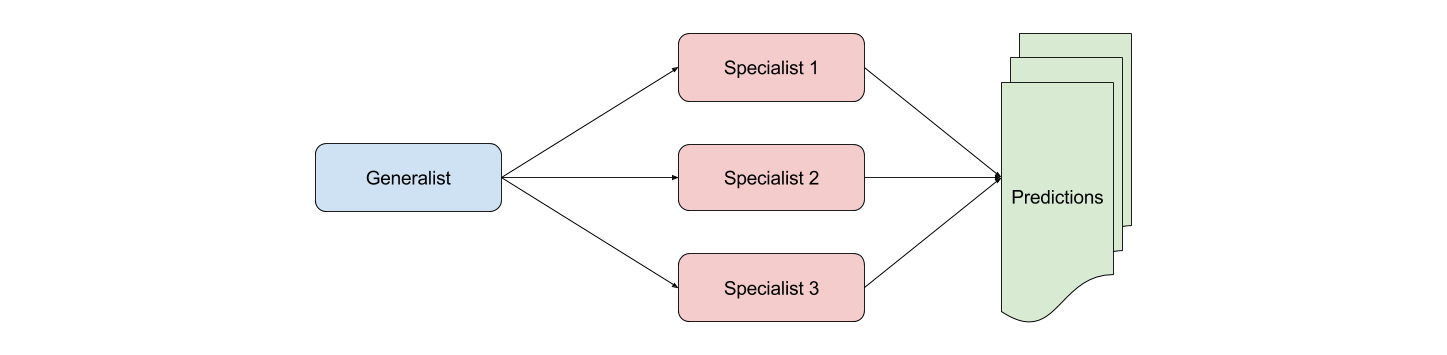
\includegraphics[width=\textwidth]{./figs/specialists.png}
\caption{An example of specialist architecture with three specialists.}
\label{fig:1}
\end{figure}

A more structured alternative to ensembling is the use of the
specialist-generalist framework. As described by \cite{bochereau1990}, a
natural analogy can be drawn from the medical field; a patient first
consults a general practitioner who provides an initial diagnosis which
is then refined by one or several specialists. In the case of
classification, the doctors are replaced by neural networks and the
final prediction is a combination of the specialists' outputs, and may
or may not include the generalist's take.

In recent years, generalist and specialists have been studied under
different circumstances. \cite{darkknowledge} used specialists to create
an efficient image classifier for a large private dataset. The final
predictions of the specialists were then used to train a reduced
classifier that achieved performance similar to the whole ensemble.
\cite{emonets} describe a multimodal approach for emotion recognition in
videos, based on specialists. Maybe closer to our work,
\cite{wardefarley} added ``auxiliary heads'' (acting as specialists) to
their baseline network, using the precomputed features for both
classification and clustering. They also underlined one of the main
advantages of using specialists; a relatively low (and parallelizable)
additional computational cost for increased performance.

\section{Clustering Algorithms}\label{clustering-algorithms}

In the generalist-specialist framework, each class is assigned to one or more
specialists. This assignment is usually done by clustering the classes into
non-overlapping sets. The goal of the clustering procedure is to optimize the
generalist vs specialist accuracy trade-off. In that sense, the algorithm must
carefully balance the classification performance of the generalist over the set
of clusters and the specialist performance within those clusters. In the case
of overlapping clusters, an additional weighting parameter for specialists can be added at
inference time.

In order to assign classes to the specialist networks, we compare
several clustering algorithms on the confusion matrix of the outputs of
the generalist. This confusion matrix is computed on a held-out
partition of the dataset. Following previous works, we started by
considering two baseline clustering algorithms, namely Lloyd's K-Means
algorithm and Spectral clustering, according to the formulation of
\cite{spectral}. In addition to those baseline algorithms, we evaluate
the performance of two novel procedures specifically designed to improve
the generalist-specialist paradigm. Those algorithms are described in
the following paragraphs, and pseudo code is given in the Appendix.

We also experimented with different ways of building the confusion matrix.
Besides the usual way of constructing a confusion matrix by accumulating all
predictions for each classes (denoted here as \emph{standard}), we tried three
alternatives:

\begin{itemize}
\itemsep1pt\parskip0pt\parsep0pt
\item
  \emph{softsum}: for each prediction, we use the raw model output
  instead of the one-hot multi-class output,
\item
  \emph{softsum pred}: just like \emph{softsum}, but only add the
  prediction output to the confusion matrix, if the class was correctly
  predicted,
\item
  \emph{softsum not pred}: like to \emph{softsum pred}, but only if
  the prediction output was incorrectly predicted.
\end{itemize}

As discussed in later sections, the influence of the confusion matrix is
minimal. Nonetheless we include them for completeness purposes.

Both of our clustering algorithms further modify the confusion matrix
$A$ by computing $CM = \textbf{A}^\top + \textbf{A}$, which symmetrizes
the matrix. We define the entries of the matrix to be the
\emph{animosity score} between two classes; given classes \emph{a} and
\emph{b}, their animosity score is found at $CM_{a, b}$. We then
initialize each cluster with non-overlapping pairs of classes yielding
maximal animosity score. Finally, we greedily select the next classes to
be added to the clusters, according to the following rules:

\begin{itemize}
\item
  In the case of \emph{greedy single} clustering, a single class
  maximizing the overall animosity score is added to the cluster
  yielding the largest averaged sum of animosity towards this class.
  This partitions the classes in clusters, building on the intuition
  that classes that are hard to distinguish should be put together.
\item
  In the case of \emph{greedy pairs} clustering, we follow the same
  strategy as in \emph{greedy single} clustering but act on pair of
  classes instead of single classes. In this case we allow the clusters
  to overlap, and one prediction might include the opinion of several
  specialists.
\end{itemize}

This process is repeated until all classes have been assigned to at
least one cluster.

\section{Experiments}\label{experiments}

We investigate the performance of the aforementioned algorithms on the
CIFAR-10 and CIFAR-100 datasets (\cite{cifar}). Both datasets contain
similar images, partitioned in 45'000 train, 5'000 validation, and
10'000 test images. They contain 10 and 100 classes respectively. For
both experiments we train the generalist network on the train set only,
and use the validation set for clustering purposes. As we are interested
in the clustering performance we do not augment nor pre-process the
images. Note that when trained on the horizontally flipped training and
validation set our baseline algorithm reaches 10.18\% and 32.22\%
misclassification error respectively, which is competitive with the
current state-of-the-art presented in \cite{allcnn}.

Following \cite{binaryconnect}, the baseline network is based on the
conclusions of \cite{vgg} and uses three pairs of batch-normalized
convolutional layers, each followed by a max-pooling layer, and two
fully-connected layers. The same model is used for specialists, whose
weights are initialized with the trained weights of the generalist.
\footnote{The code for these experiments is freely available online at
  \href{http://www.github.com/seba-1511/specialists}.}
One major departure from the work of \cite{darkknowledge} is that our
specialists are predicting over the same classes as the generalist,
i.e.~we do not merge all classes outside of the cluster into a unique
one. With regards to the generalist, a specialist is only biased towards
a subset of the classes, since it has been fine-tuned to perform well on
those ones.

\subsection{CIFAR-10}\label{cifar-10}

\begin{longtable}[c]{@{}lllll@{}}
\toprule\addlinespace
Results & standard & soft sum & soft sum pred & soft sum not pred
\\\addlinespace
\midrule\endhead
spectral & (0.7046, 2) & (0.7719, 2) & (0.6989, 2) & (0.706, 2)
\\\addlinespace
greedy singles & (0.5873, 2) & (0.5049, 2) & (0.5139, 3) & (0.5873, 2)
\\\addlinespace
kmeans & (0.8202, 2) & (0.8202, 2) & (0.8202, 2) & (0.8202, 2)
\\\addlinespace
greedy pairs & (0.8835, 2) & (0.8835, 2) & (0.8727, 3) & (0.8835, 2)
\\\addlinespace
\bottomrule
\addlinespace
\caption{Experiment results for CIFAR-10}
\end{longtable}

For CIFAR-10 experiments, we considered up to five clusters, and all of the
possible combinations of confusion matrix and clustering algorithms. The
results for this experiments are reported in Table 1. For each clustering
algorithm and confusion matrix type we report first the obtained accuracy, and
then the number of clusters to reach it.

%\begin{table}
%\caption{Experiment results for CIFAR-10}
%\label{tab:1}       % Give a unique label
%\begin{tabular}{p{3.2cm}p{2.0cm}p{2.0cm}p{2.0cm}p{2.0cm}}
%\hline\noalign{\smallskip}
%Clustering Algorithm & standard & softsum & softsum pred & softsum not pred \\
%%\noalign{\smallskip}\svhline\noalign{\smallskip}
%spectral & (0.7046, 2) & (0.7719, 2) & (0.6989, 2) & (0.706, 2) \\
%greedy singles & (0.5873, 2) & (0.5049, 2) & (0.5139, 3) & (0.5873, 2) \\
%kmeans & (0.8202, 2) & (0.8202, 2) & (0.8202, 2) & (0.8202, 2) \\
%greedy pairs & (0.8835, 2) & (0.8835, 2) & (0.8727, 3) & (0.8835, 2) \\
%%\noalign{\smallskip}\hline\noalign{\smallskip}
%\end{tabular}
%\end{table}


Interestingly, the choice of confusion matrix has only a limited impact
on the overall performance, indicating that the emphasis should be put
on the clustering algorithm. We notice that clustering with greedy pairs
consistently yields better scores. However none of the specialist
experiments is able to improve on the baseline, suggesting that
specialists might not be the framework of choice when dealing with a
small number of classes.

\subsection{CIFAR-100}\label{cifar-100}

For CIFAR-100 we performed the exact same experiment as for CIFAR-10 but used
more specialists, the largest experiments involving 28 clusters. The results
are shown in Table 2. Again, we report the obtained accuracy and the number of
clusters for each clustering algorithm and confusion matrix type.

%\begin{table}
%\caption{Experiment results for CIFAR-100}
%\label{tab:2}       % Give a unique label
%\begin{tabular}{p{3.2cm}p{2.0cm}p{2.0cm}p{2.0cm}p{2.0cm}}
%\hline\noalign{\smallskip}
%Clustering Algorithm & standard & softsum & softsum pred & softsum not pred \\
%%\noalign{\smallskip}\svhline\noalign{\smallskip}
%spectral &  (0.2632, 2) & (0.1769, 2) & (0.408, 4) & (0.2749, 2) \\
%greedy singles & (0.4112, 2) & (0.4356, 2) & (0.3851, 2) & (0.4308, 2) \\
%kmeans & (0.5123, 2) & (0.5123, 2) & (0.2058, 4) & (0.6141, 2) \\
%greedy pairs & (0.6407, 2) & (0.6375, 4) & (0.6408, 4) & (0.6413, 4) \\
%\noalign{\smallskip}\hline\noalign{\smallskip}
%\end{tabular}
%\end{table}


\begin{longtable}[c]{@{}lllll@{}}
\toprule\addlinespace
Results & standard & soft sum & soft sum pred & soft sum not pred
\\\addlinespace
\midrule\endhead
spectral & (0.5828, 2) & (0.5713, 2) & (0.5755, 2) & (0.5795, 3)
\\\addlinespace
greedy singles & (0.3834, 2) & (0.3733, 2) & (0.3803, 2) & (0.3551, 2)
\\\addlinespace
kmeans & (0.5908, 2) & (0.5618, 2) & (0.5820, 3) & (0.5876, 2)
\\\addlinespace
greedy pairs & (0.6141, 6) & (0.5993, 6) & (0.6111, 6) & (0.607, 6)
\\\addlinespace
\bottomrule
\addlinespace
\caption{Experiment results for CIFAR-100}
\end{longtable}

Similarly to CIFAR-10, we observe that greedy pairs clustering
outperforms the other clustering techniques, and that the different
types of confusion matrix have a limited influence on the final score.
We also notice that fewer clusters tend to work better. Finally, and
unlike the results for CIFAR-10, some of the specialists are able to
improve upon the generalist, which confirms our intuition that
specialists are better suited to problems involving numerous output
classes.

We suggest the following explanation for the improved performance of
greedy pairs is the following. Allowing clusters to overlap leads to the
assignment of difficult classes to multiple specialists. At inference
time, more networks will influence the final prediction which is
analogous to building a larger ensemble for difficult classes.

\section{Conclusion and Future Work}\label{conclusion-and-future-work}

We introduce a novel clustering algorithm for the specialist-generalist
framework, which is able to consistently outperform other techniques. We
also provide a preliminary study of the different factors coming into
play when dealing with specialists, and conclude that the choice of
confusion matrix from our proposed set only has little impact on the
final classification outcome.

Despite our encouraging results with clustering techniques, no one of
our specialists-based experiments came close to compete with the
generalist model trained on the entire train and validation set. This
was a surprising outcome and we suppose that this effect comes from the
size of the datasets. In both cases, 5'000 images corresponds to 10\% of
the original training set and removing that many training examples has a
drastic effect on both generalists and specialists. All the more so
since we are not using any kind of data augmentation techniques, which
could have moderated this downside. An obvious future step is to
validate the presented ideas on a much larger dataset such as
Imagenet \cite{imagenet} where splitting the train set would not hurt the train
score as much.

%\acknowledgement
\subsubsection{Acknowledgments}

We would like to thank Greg Ver Steeg, Gabriel Pereyra, and Pranav Rajpurkar for their comments and advices. We also thank Nervana Systems
for providing GPUs as well as their help with their deep learning
framework.

\section{Appendix}\label{appendix}

%\subsection{Greedy Pairs Pseudo Code}\label{greedy-pairs-pseudo-code}

\begin{algorithm}[H]
    \caption{Greedy Pairs Clustering}
    \label{greedy_pairs}
    \begin{algorithmic}[1] % The number tells where the line numbering should start
        \Procedure{GreedyPairs}{$M,N$} \Comment{Confusion matrix M, number of clusters N}
            \State $M\gets M + M^T$
            \State Initialize N clusters with non-overlapping pairs maximizing the entries of M.
            \While{every class has not been assigned}
                \State Get the next pair $(a, b)$ maximizing the entry in M
                \State cluster = $\underset{\text{c in clusters}}{\mathrm{argmin}}$(Animosity(a, c) + Animosity(b, c))
                \State Assign(cluster, a, b)
            \EndWhile\label{euclidendwhile}
            \State \textbf{return} clusters
        \EndProcedure
    \end{algorithmic}
\end{algorithm}

%Note: A python implementation of both greedy pairs and greedy single can
%be found at \url{http://www.github.com/seba-1511/specialists}.

%%%%%%%%%%%%%%%%%%%%%%%%% referenc.tex %%%%%%%%%%%%%%%%%%%%%%%%%%%%%%
% sample references
% %
% Use this file as a template for your own input.
%
%%%%%%%%%%%%%%%%%%%%%%%% Springer-Verlag %%%%%%%%%%%%%%%%%%%%%%%%%%
%
% BibTeX users please use
 %\bibliographystyle{}
 %\bibliography{}
%
%\biblstarthook{References may be \textit{cited} in the text either by number (preferred) or by author/year.\footnote{Make sure that all references from the list are cited in the text. Those not cited should be moved to a separate \textit{Further Reading} section or chapter.} The reference list should ideally be \textit{sorted} in alphabetical order -- even if reference numbers are used for the their citation in the text. If there are several works by the same author, the following order should be used: 
%\begin{enumerate}
%\item all works by the author alone, ordered chronologically by year of publication
%\item all works by the author with a coauthor, ordered alphabetically by coauthor
%\item all works by the author with several coauthors, ordered chronologically by year of publication.
%\end{enumerate}
%The \textit{styling} of references\footnote{Always use the standard abbreviation of a journal's name according to the ISSN \textit{List of Title Word Abbreviations}, see \url{http://www.issn.org/en/node/344}} depends on the subject of your book:
%\begin{itemize}
%\item The \textit{two} recommended styles for references in books on \textit{mathematical, physical, statistical and computer sciences} are depicted in ~\cite{science-contrib, science-online, science-mono, science-journal, science-DOI} and ~\cite{phys-online, phys-mono, phys-journal, phys-DOI, phys-contrib}.
%\item Examples of the most commonly used reference style in books on \textit{Psychology, Social Sciences} are~\cite{psysoc-mono, psysoc-online,psysoc-journal, psysoc-contrib, psysoc-DOI}.
%\item Examples for references in books on \textit{Humanities, Linguistics, Philosophy} are~\cite{humlinphil-journal, humlinphil-contrib, humlinphil-mono, humlinphil-online, humlinphil-DOI}.
%\item Examples of the basic Springer style used in publications on a wide range of subjects such as \textit{Computer Science, Economics, Engineering, Geosciences, Life Sciences, Medicine, Biomedicine} are ~\cite{basic-contrib, basic-online, basic-journal, basic-DOI, basic-mono}. 
%\end{itemize}
%}

\begin{thebibliography}{99.}%


    \bibitem{bochereau1990}Bochereau, Laurent, and Bourgine, Paul. A Generalist-Specialist Paradigm for
Multilayer Neural Networks. Neural Networks, 1990.


\bibitem{binaryconnect}Courbariaux, Matthieu, Bengio, Yoshua, and David, Jean-Pierre. BinaryConnect:
Training Deep Neural Networks with Binary Weights during Propagations. NIPS,
2015.


\bibitem{galaxy}Dieleman, Sander, Willett, Kyle W., and Dambre, Joni. Rotation-invarient
convolutional neural networks for galaxy morphology prediction. Oxford Journals,
2015.


\bibitem{deepspeech2}Hannun, Awni, Case, Carl, Casper, Jared, Catanzaro, Bryan, Diamos, Greg, Elsen,
Erich, Prenger, Ryan, Satheesh, Sanjeev, Sengupta, Shubho, Coates, Adam, and Ng,
Andrew Y. Deep Speach: Scaling up end-to-end speech recognition. Arxiv Preprint,
2014.


\bibitem{darkknowledge}Hinton, Geoffrey E., Vinyals, Oriol, and Dean, Jeff. Distilling th Knowledge in
a Neural Network. NIPS 2014 Deep Learning Workshop.


\bibitem{emonets}Kahou, Samira Ebrahimi, Bouthiller, Xavier, Lamblin, Pascal, Gulcehre, Caglar,
Michalski, Vincent, Konda, Kishore, Jean, S�bastien, Froumenty, Pierre, Dauphin,
Yann, Boulanger-Lewandowski, Nicolas, Ferrari, Raul Chandias, Mirza, Mehdi,
Warde-Farley, David, Courville, Aaron, Vincent, Pascal, Memisevic, Roland, Pal,
Christopher, and Bengio, Yoshua. EmoNets: Multimodal deep learning approaches
for emation recofnition in video. Journal on Mutlimodal User Interfaces, 2015.


\bibitem{cifar}Krizhevsky, Alex. Learning Multiple Layers of Features from Tiny Images. 2009.


\bibitem{spectral}Ng, Andrew Y., Jordan, Micheal I., Weiss, Yair. On spectral clustering: Analysis
and an algorithm. NIPS 2002.


\bibitem{imagenet}Russakovsky, Olga, Deng, Jia, Su, Hao, Krause, Jonathan, Satheesh, Sanjeev, Ma,
Sean, huang, Zhiheng, Karpathy, Andrej, Khosla, Aditya, Bernstain, Michael,
Berg, Alexander C., and Fei-Fei, Li. ImageNet Large Scale Visual Recognition
Challenge. International Journal of Computer Vision, 2015.


\bibitem{vgg}Simonyan, Karen and Zisserman, Andrew. Very Deep Convolutional Networks for
Large-Scale Image Recognition. International Conference on Learning
Representations, 2015.


\bibitem{allcnn}Springenberg, Jost Tobias, Dosovitskiy, Alexey, Brox, Thomas, and Riedmiller,
Martin. Striving for Simplicity: The All Convolutional Net. International
Conference on Learning Representations Workshop, 2015.


\bibitem{seq2seq}Sutskever, Ilya, Vinyals, Oriol, and Le, Quoc V. Sequence to Sequence Learning with
Neural Networks. Arxiv Preprint, 2014.


\bibitem{inception}Szegedy, Christian, Liu, Wei, Jia, Yangqing, Sermanet, Pierre, Reed, Scott,
Anguelov, Dragomir, Erhan, Dumitru, Vanhoucke, Vincent, and Rabinovich, Andrew.
Going deeper with convolutions. Arxiv Preprint, 2014.


\bibitem{wardefarley}Warde-Farley, David, Rabinovich, Andrew, and  Anguelov, Dragomir. Self-Informed
Neural Networks Structure Learning. International Conference on Representations
Learning, 2015.

%@inproceedings{bochereau1990,
  %title={A generalist-specialist paradigm for multilayer neural networks},
  %author={Bochereau, Laurent and Bourgine, Paul},
  %booktitle={Neural Networks, 1990., 1990 IJCNN International Joint Conference on},
  %pages={87--91},
  %year={1990},
  %organization={IEEE}
%}

%@inproceedings{binaryconnect,
  %title={BinaryConnect: Training Deep Neural Networks with binary weights during propagations},
  %author={Courbariaux, Matthieu and Bengio, Yoshua and David, Jean-Pierre},
  %booktitle={Advances in Neural Information Processing Systems},
  %pages={3105--3113},
  %year={2015}
%}

%@article{galaxy,
  %title={Rotation-invariant convolutional neural networks for galaxy morphology prediction},
  %author={Dieleman, Sander and Willett, Kyle W and Dambre, Joni},
  %journal={Monthly Notices of the Royal Astronomical Society},
  %volume={450},
  %number={2},
  %pages={1441--1459},
  %year={2015},
  %publisher={Oxford University Press}
%}

%@article{deepspeech2,
  %title={Deep Speech 2: End-to-End Speech Recognition in English and Mandarin},
  %author={Amodei, Dario and Anubhai, Rishita and Battenberg, Eric and Case, Carl and Casper, Jared and Catanzaro, Bryan and Chen, Jingdong and Chrzanowski, Mike and Coates, Adam and Diamos, Greg and others},
  %journal={arXiv preprint arXiv:1512.02595},
  %year={2015}
%}

%@article{darkknowledge,
  %title={Distilling the knowledge in a neural network},
  %author={Hinton, Geoffrey and Vinyals, Oriol and Dean, Jeff},
  %journal={arXiv preprint arXiv:1503.02531},
  %year={2015}
%}

%@article{emonets,
  %title={Emonets: Multimodal deep learning approaches for emotion recognition in video},
  %author={Kahou, Samira Ebrahimi and Bouthillier, Xavier and Lamblin, Pascal and Gulcehre, Caglar and Michalski, Vincent and Konda, Kishore and Jean, S{\'e}bastien and Froumenty, Pierre and Dauphin, Yann and Boulanger-Lewandowski, Nicolas and others},
  %journal={Journal on Multimodal User Interfaces},
  %pages={1--13},
  %publisher={Springer}
%}

%@misc{cifar,
  %title={Learning multiple layers of features from tiny images},
  %author={Krizhevsky, Alex},
  %year={2009},
  %publisher={Citeseer}
%}

%@article{spectral,
  %title={On Spectral Clustering: Analysis and an algorithm},
  %author={Ng, Andrew Y and Jordan, Michael I and Weiss, Yair}
%}

%@article{imagenet,
  %title={Imagenet large scale visual recognition challenge},
  %author={Russakovsky, Olga and Deng, Jia and Su, Hao and Krause, Jonathan and Satheesh, Sanjeev and Ma, Sean and Huang, Zhiheng and Karpathy, Andrej and Khosla, Aditya and Bernstein, Michael and others},
  %journal={International Journal of Computer Vision},
  %volume={115},
  %number={3},
  %pages={211--252},
  %year={2015},
  %publisher={Springer}
%}

%@article{vgg,
  %title={Very deep convolutional networks for large-scale image recognition},
  %author={Simonyan, Karen and Zisserman, Andrew},
  %journal={arXiv preprint arXiv:1409.1556},
  %year={2014}
%}

%@article{allcnn,
  %title={Striving for simplicity: The all convolutional net},
  %author={Springenberg, Jost Tobias and Dosovitskiy, Alexey and Brox, Thomas and Riedmiller, Martin},
  %journal={arXiv preprint arXiv:1412.6806},
  %year={2014}
%}

%@inproceedings{seq2seq,
  %title={Sequence to sequence learning with neural networks},
  %author={Sutskever, Ilya and Vinyals, Oriol and Le, Quoc V},
  %booktitle={Advances in neural information processing systems},
  %pages={3104--3112},
  %year={2014}
%}

%@inproceedings{inception,
  %title={Going deeper with convolutions},
  %author={Szegedy, Christian and Liu, Wei and Jia, Yangqing and Sermanet, Pierre and Reed, Scott and Anguelov, Dragomir and Erhan, Dumitru and Vanhoucke, Vincent and Rabinovich, Andrew},
  %booktitle={Proceedings of the IEEE Conference on Computer Vision and Pattern Recognition},
  %pages={1--9},
  %year={2015}
%}

%@article{wardefarley,
  %title={Self-informed neural network structure learning},
  %author={Warde-Farley, David and Rabinovich, Andrew and Anguelov, Dragomir},
  %journal={arXiv preprint arXiv:1412.6563},
  %year={2014}
%}




% and use \bibitem to create references.
%
% Use the following syntax and markup for your references if 
% the subject of your book is from the field 
% "Mathematics, Physics, Statistics, Computer Science"
%
% Contribution 
%\bibitem{science-contrib} Broy, M.: Software engineering --- from auxiliary to key technologies. In: Broy, M., Dener, E. (eds.) Software Pioneers, pp. 10-13. Springer, Heidelberg (2002)
%%
%% Online Document
%\bibitem{science-online} Dod, J.: Effective substances. In: The Dictionary of Substances and Their Effects. Royal Society of Chemistry (1999) Available via DIALOG. \\
%\url{http://www.rsc.org/dose/title of subordinate document. Cited 15 Jan 1999}
%%
%% Monograph
%\bibitem{science-mono} Geddes, K.O., Czapor, S.R., Labahn, G.: Algorithms for Computer Algebra. Kluwer, Boston (1992) 
%%
%% Journal article
%\bibitem{science-journal} Hamburger, C.: Quasimonotonicity, regularity and duality for nonlinear systems of partial differential equations. Ann. Mat. Pura. Appl. \textbf{169}, 321--354 (1995)
%%
%% Journal article by DOI
%\bibitem{science-DOI} Slifka, M.K., Whitton, J.L.: Clinical implications of dysregulated cytokine production. J. Mol. Med. (2000) doi: 10.1007/s001090000086 
%%
%\bigskip

% Use the following (APS) syntax and markup for your references if 
% the subject of your book is from the field 
% "Mathematics, Physics, Statistics, Computer Science"
%
% Online Document
%\bibitem{phys-online} J. Dod, in \textit{The Dictionary of Substances and Their Effects}, Royal Society of Chemistry. (Available via DIALOG, 1999), 
%\url{http://www.rsc.org/dose/title of subordinate document. Cited 15 Jan 1999}
%%
%% Monograph
%\bibitem{phys-mono} H. Ibach, H. L\"uth, \textit{Solid-State Physics}, 2nd edn. (Springer, New York, 1996), pp. 45-56 
%%
%% Journal article
%\bibitem{phys-journal} S. Preuss, A. Demchuk Jr., M. Stuke, Appl. Phys. A \textbf{61}
%%
%% Journal article by DOI
%\bibitem{phys-DOI} M.K. Slifka, J.L. Whitton, J. Mol. Med., doi: 10.1007/s001090000086
%%
%% Contribution 
%\bibitem{phys-contrib} S.E. Smith, in \textit{Neuromuscular Junction}, ed. by E. Zaimis. Handbook of Experimental Pharmacology, vol 42 (Springer, Heidelberg, 1976), p. 593
%%
%\bigskip
%%
%% Use the following syntax and markup for your references if 
%% the subject of your book is from the field 
%% "Psychology, Social Sciences"
%%
%%
%% Monograph
%\bibitem{psysoc-mono} Calfee, R.~C., \& Valencia, R.~R. (1991). \textit{APA guide to preparing manuscripts for journal publication.} Washington, DC: American Psychological Association.
%%
%% Online Document
%\bibitem{psysoc-online} Dod, J. (1999). Effective substances. In: The dictionary of substances and their effects. Royal Society of Chemistry. Available via DIALOG. \\
%\url{http://www.rsc.org/dose/Effective substances.} Cited 15 Jan 1999.
%%
%% Journal article
%\bibitem{psysoc-journal} Harris, M., Karper, E., Stacks, G., Hoffman, D., DeNiro, R., Cruz, P., et al. (2001). Writing labs and the Hollywood connection. \textit{J Film} Writing, 44(3), 213--245.
%%
%% Contribution 
%\bibitem{psysoc-contrib} O'Neil, J.~M., \& Egan, J. (1992). Men's and women's gender role journeys: Metaphor for healing, transition, and transformation. In B.~R. Wainrig (Ed.), \textit{Gender issues across the life cycle} (pp. 107--123). New York: Springer.
%%
%% Journal article by DOI
%\bibitem{psysoc-DOI}Kreger, M., Brindis, C.D., Manuel, D.M., Sassoubre, L. (2007). Lessons learned in systems change initiatives: benchmarks and indicators. \textit{American Journal of Community Psychology}, doi: 10.1007/s10464-007-9108-14.
%%
%%
%% Use the following syntax and markup for your references if 
%% the subject of your book is from the field 
%% "Humanities, Linguistics, Philosophy"
%%
%\bigskip
%%
%% Journal article
%\bibitem{humlinphil-journal} Alber John, Daniel C. O'Connell, and Sabine Kowal. 2002. Personal perspective in TV interviews. \textit{Pragmatics} 12:257--271
%%
%% Contribution 
%\bibitem{humlinphil-contrib} Cameron, Deborah. 1997. Theoretical debates in feminist linguistics: Questions of sex and gender. In \textit{Gender and discourse}, ed. Ruth Wodak, 99--119. London: Sage Publications.
%%
%% Monograph
%\bibitem{humlinphil-mono} Cameron, Deborah. 1985. \textit{Feminism and linguistic theory.} New York: St. Martin's Press.
%%
%% Online Document
%\bibitem{humlinphil-online} Dod, Jake. 1999. Effective substances. In: The dictionary of substances and their effects. Royal Society of Chemistry. Available via DIALOG. \\
%http://www.rsc.org/dose/title of subordinate document. Cited 15 Jan 1999
%%
%% Journal article by DOI
%\bibitem{humlinphil-DOI} Suleiman, Camelia, Daniel C. O�Connell, and Sabine Kowal. 2002. `If you and I, if we, in this later day, lose that sacred fire...�': Perspective in political interviews. \textit{Journal of Psycholinguistic Research}. doi: 10.1023/A:1015592129296.
%%
%%
%%
%\bigskip
%%
%%
%% Use the following syntax and markup for your references if 
%% the subject of your book is from the field 
%% "Computer Science, Economics, Engineering, Geosciences, Life Sciences"
%%
%%
%% Contribution 
%\bibitem{basic-contrib} Brown B, Aaron M (2001) The politics of nature. In: Smith J (ed) The rise of modern genomics, 3rd edn. Wiley, New York 
%%
%% Online Document
%\bibitem{basic-online} Dod J (1999) Effective Substances. In: The dictionary of substances and their effects. Royal Society of Chemistry. Available via DIALOG. \\
%\url{http://www.rsc.org/dose/title of subordinate document. Cited 15 Jan 1999}
%%
%% Journal article by DOI
%\bibitem{basic-DOI} Slifka MK, Whitton JL (2000) Clinical implications of dysregulated cytokine production. J Mol Med, doi: 10.1007/s001090000086
%%
%% Journal article
%\bibitem{basic-journal} Smith J, Jones M Jr, Houghton L et al (1999) Future of health insurance. N Engl J Med 965:325--329
%%
%% Monograph
%\bibitem{basic-mono} South J, Blass B (2001) The future of modern genomics. Blackwell, London 
%
\end{thebibliography}


%\begin{thebibliography}
%\bibliographystyle{apalike}
%\bibliographystyle{}

%\bibliography{biblio}

\begin{thebibliography}{99.}%


    \bibitem{bochereau1990}Bochereau, Laurent, and Bourgine, Paul. A Generalist-Specialist Paradigm for
Multilayer Neural Networks. Neural Networks, 1990.


\bibitem{binaryconnect}Courbariaux, Matthieu, Bengio, Yoshua, and David, Jean-Pierre. BinaryConnect:
Training Deep Neural Networks with Binary Weights during Propagations. NIPS,
2015.


\bibitem{galaxy}Dieleman, Sander, Willett, Kyle W., and Dambre, Joni. Rotation-invarient
convolutional neural networks for galaxy morphology prediction. Oxford Journals,
2015.


\bibitem{deepspeech2}Hannun, Awni, Case, Carl, Casper, Jared, Catanzaro, Bryan, Diamos, Greg, Elsen,
Erich, Prenger, Ryan, Satheesh, Sanjeev, Sengupta, Shubho, Coates, Adam, and Ng,
Andrew Y. Deep Speach: Scaling up end-to-end speech recognition. Arxiv Preprint,
2014.


\bibitem{darkknowledge}Hinton, Geoffrey E., Vinyals, Oriol, and Dean, Jeff. Distilling th Knowledge in
a Neural Network. NIPS 2014 Deep Learning Workshop.


\bibitem{emonets}Kahou, Samira Ebrahimi, Bouthiller, Xavier, Lamblin, Pascal, Gulcehre, Caglar,
Michalski, Vincent, Konda, Kishore, Jean, Sébastien, Froumenty, Pierre, Dauphin,
Yann, Boulanger-Lewandowski, Nicolas, Ferrari, Raul Chandias, Mirza, Mehdi,
Warde-Farley, David, Courville, Aaron, Vincent, Pascal, Memisevic, Roland, Pal,
Christopher, and Bengio, Yoshua. EmoNets: Multimodal deep learning approaches
for emation recofnition in video. Journal on Mutlimodal User Interfaces, 2015.


\bibitem{cifar}Krizhevsky, Alex. Learning Multiple Layers of Features from Tiny Images. 2009.


\bibitem{spectral}Ng, Andrew Y., Jordan, Micheal I., Weiss, Yair. On spectral clustering: Analysis
and an algorithm. NIPS 2002.


\bibitem{imagenet}Russakovsky, Olga, Deng, Jia, Su, Hao, Krause, Jonathan, Satheesh, Sanjeev, Ma,
Sean, huang, Zhiheng, Karpathy, Andrej, Khosla, Aditya, Bernstain, Michael,
Berg, Alexander C., and Fei-Fei, Li. ImageNet Large Scale Visual Recognition
Challenge. International Journal of Computer Vision, 2015.


\bibitem{vgg}Simonyan, Karen and Zisserman, Andrew. Very Deep Convolutional Networks for
Large-Scale Image Recognition. International Conference on Learning
Representations, 2015.


\bibitem{allcnn}Springenberg, Jost Tobias, Dosovitskiy, Alexey, Brox, Thomas, and Riedmiller,
Martin. Striving for Simplicity: The All Convolutional Net. International
Conference on Learning Representations Workshop, 2015.


\bibitem{seq2seq}Sutskever, Ilya, Vinyals, Oriol, and Le, Quoc V. Sequence to Sequence Learning with
Neural Networks. Arxiv Preprint, 2014.


\bibitem{inception}Szegedy, Christian, Liu, Wei, Jia, Yangqing, Sermanet, Pierre, Reed, Scott,
Anguelov, Dragomir, Erhan, Dumitru, Vanhoucke, Vincent, and Rabinovich, Andrew.
Going deeper with convolutions. Arxiv Preprint, 2014.


\bibitem{wardefarley}Warde-Farley, David, Rabinovich, Andrew, and  Anguelov, Dragomir. Self-Informed
Neural Networks Structure Learning. International Conference on Representations
Learning, 2015.
\end{thebibliography}

%\end{multicols}
\end{document}
%\abstract
%With the recent advances in deep neural networks, several experiments
%involved the generalist-specialist paradigm for classification. However,
%until now no formal study compared the performance of different
%clustering algorithms for class assignment. In this paper we perform
%such a study, suggest slight modifications to the clustering procedures,
%and propose a novel algorithm designed to optimize the performance of of
%the specialist-generalist classification system. Our experiments on the
%CIFAR-10 and CIFAR-100 datasets allow us to investigate situations for
%varying number of classes on similar data. We find that our
%\emph{greedy\_pairs} clustering algorithm consistently outperforms other
%alternatives, while the choice of the confusion matrix has little impact
%on the final performance.

%\section{Introduction}\label{introduction}

%Designing an efficient classification system using deep neural networks
%is a complicated task, which often use a multitude of models arranged in
%ensembles. (\cite{galaxy}, \cite{vgg}) Those ensembles often lead to
%state-of-the-art results on a wide range of different tasks such as
%image classification (\cite{inception}), speech recognition
%(\cite{deepspeech2}), and machine translation (\cite{seq2seq}). The
%models are trained independently and in parallel, and different
%techniques can be used to merge their predictions.

%\begin{figure}[htbp]
%\centering
%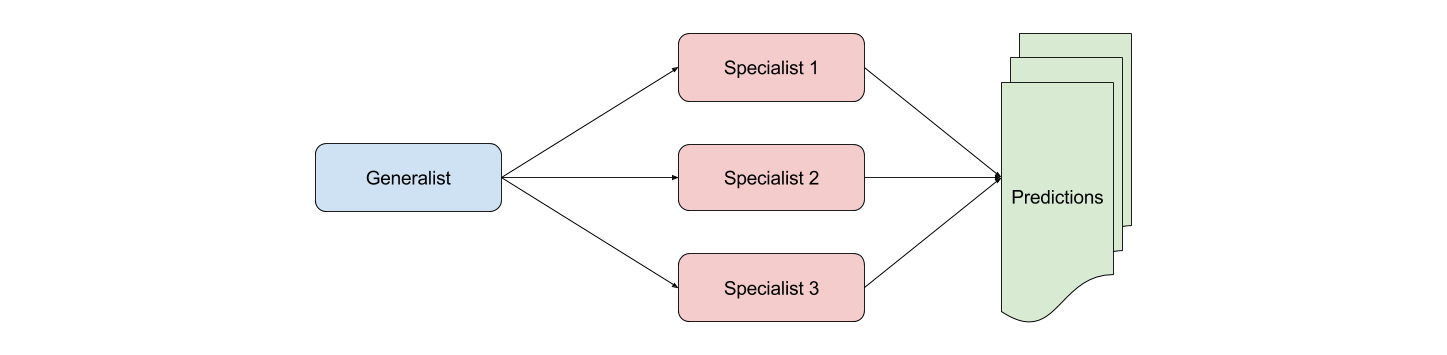
\includegraphics{./figs/specialists.png}
%\caption{An example of specialist architecture with three specialists}
%\end{figure}

%A more structured alternative to ensembling is the use of the
%specialist-generalist framework. As described by \cite{bochereau1990}, a
%natural analogy can be drawn from the medical field; a patient first
%consults a general practitioner who provides an initial diagnosis which
%is then refined by one or several specialists. In the case of
%classification, the doctors are replaced by neural networks and the
%final prediction is a combination of the specialists' outputs, and may
%or may not include the generalist's take.

%In recent years, generalist and specialists have been studied under
%different circumstances. \cite{darkknowledge} used specialists to create
%an efficient image classifier for a large private dataset. The final
%predictions of the specialists were then used to train a reduced
%classifier that achieved performance similar to the whole ensemble.
%\cite{emonets} describe a multimodal approach for emotion recognition in
%videos, based on specialists. Maybe closer to our work,
%\cite{wardefarley} added ``auxiliary heads'' (acting as specialists) to
%their baseline network, using the precomputed features for both
%classification and clustering. They also underlined one of the main
%advantages of using specialists; a relatively low (and parallelizable)
%additional computational cost for increased performance.

%\section{Clustering Algorithms}\label{clustering-algorithms}

%In order to assign classes to the specialist networks, we compare
%several clustering algorithms on the confusion matrix of the outputs of
%the generalist. This confusion matrix is computed on a held-out
%partition of the dataset. Following previous works, we started by
%considering two baseline clustering algorithms, namely Lloyd's K-Means
%algorithm and Spectral clustering, according to the formulation of
%\cite{spectral}. In addition to those baseline algorithms, we evaluate
%the performance of two novel procedures specifically designed to improve
%the generalist-specialist paradigm. Those algorithms are described in
%the following paragraphs, and pseudo code is given in the Appendix.

%We also experimented with different ways of building the confusion
%matrix. Besides the usual way (denoted here as \emph{standard}) we tried
%three alternatives:

%\begin{itemize}
%\itemsep1pt\parskip0pt\parsep0pt
%\item
  %\emph{soft sum}: for each prediction, we use the raw model output
  %instead of the one-hot multi-class output,
%\item
  %\emph{soft sum pred}: just like \emph{soft sum}, but only add the
  %prediction output to the confusion matrix, if the class was correctly
  %predicted,
%\item
  %\emph{soft sum not pred}: like to \emph{soft sum pred}, but only if
  %the prediction output was incorrectly predicted.
%\end{itemize}

%As discussed in later sections, the influence of the confusion matrix is
%minimal. Nonetheless we include them for completeness purposes.

%Both of our clustering algorithms further modify the confusion matrix
%$A$ by computing $CM = \textbf{A}^\top + \textbf{A}$, which symmetrizes
%the matrix. We define the entries of the matrix to be the
%\emph{animosity score} between two classes; given classes \emph{a} and
%\emph{b}, their animosity score is found at $CM_{a, b}$. We then
%initialize each cluster with non-overlapping pairs of classes yielding
%maximal animosity score. Finally, we greedily select the next classes to
%be added to the clusters, according to the following rules:

%\begin{itemize}
%\item
  %In the case of \emph{greedy single} clustering, a single class
  %maximizing the overall animosity score is added to the cluster
  %yielding the largest averaged sum of animosity towards this class.
  %This partitions the classes in clusters, building on the intuition
  %that classes that are hard to distinguish should be put together.
%\item
  %In the case of \emph{greedy pairs} clustering, we follow the same
  %strategy as in \emph{greedy single} clustering but act on pair of
  %classes instead of single classes. In this case we allow the clusters
  %to overlap, and one prediction might include the opinion of several
  %specialists.
%\end{itemize}

%This process is repeated until all classes have been assigned to at
%least one cluster.

%\section{Experiments}\label{experiments}

%We investigate the performance of the aforementioned algorithms on the
%CIFAR-10 and CIFAR-100 datasets (\cite{cifar}). Both datasets contain
%similar images, partitioned in 45'000 train, 5'000 validation, and
%10'000 test images. They contain 10 and 100 classes respectively. For
%both experiments we train the generalist network on the train set only,
%and use the validation set for clustering purposes. As we are interested
%in the clustering performance we did not augment nor pre-process the
%images. Note that when trained on the horizontally flipped training and
%validation set our baseline algorithm reaches 10.18\% and 32.22\%
%misclassification error respectively, which is competitive with the
%current state-of-the-art presented in \cite{allcnn}.

%Following \cite{binaryconnect}, the baseline network is based on the
%conclusions of \cite{vgg} and uses three pairs of batch-normalized
%convolutional layers, each followed by a max-pooling layer, and two
%fully-connected layers. The same model is used for specialists, whose
%weights are initialized with the trained weights of the generalist.
%\footnote{The code for those experiments, is freely available online at
  %\href{http://www.github.com/seba-1511/specialists}{github.com/seba-1511/specialists}.}
%One major departure from the work of \cite{darkknowledge} is that our
%specialists are predicting over the same classes as the generalist,
%i.e.~we do not merge all classes outside of the cluster into a unique
%one. With regards to the generalist, a specialist is only biased towards
%a subset of the classes, since it has been fine-tuned to perform well on
%those ones.

%\subsection{CIFAR-10}\label{cifar-10}

%For CIFAR-10 experiments, we considered up to five clusters, and all of
%the possible combinations of confusion matrix and clustering algorithms.
%The results for this experiments are reported in Table 1.

%\begin{longtable}[c]{@{}lllll@{}}
%\toprule\addlinespace
%Results & standard & soft sum & soft sum pred & soft sum not pred
%\\\addlinespace
%\midrule\endhead
%spectral & (0.7046, 2) & (0.7719, 2) & (0.6989, 2) & (0.706, 2)
%\\\addlinespace
%greedy singles & (0.5873, 2) & (0.5049, 2) & (0.5139, 3) & (0.5873, 2)
%\\\addlinespace
%kmeans & (0.8202, 2) & (0.8202, 2) & (0.8202, 2) & (0.8202, 2)
%\\\addlinespace
%greedy pairs & (0.8835, 2) & (0.8835, 2) & (0.8727, 3) & (0.8835, 2)
%\\\addlinespace
%\bottomrule
%\addlinespace
%\caption{Experiment results for CIFAR-10}
%\end{longtable}

%Interestingly, the choice of confusion matrix has only a limited impact
%on the overall performance, indicating that the emphasis should be put
%on the clustering algorithm. We notice that clustering with greedy pairs
%consistently yields better scores. However none of the specialist
%experiments is able to improve on the baseline, suggesting that
%specialists might not be the framework of choice when dealing with a
%small number of classes.

%\subsection{CIFAR-100}\label{cifar-100}

%For CIFAR-100 we performed the exact same experiment as for CIFAR-10 but
%used more specialists, the largest experiments involving 28 clusters.
%The results are shown in Table 2.

%\begin{longtable}[c]{@{}lllll@{}}
%\toprule\addlinespace
%Results & standard & soft sum & soft sum pred & soft sum not pred
%\\\addlinespace
%\midrule\endhead
%spectral & (0.5828, 2) & (0.5713, 2) & (0.5755, 2) & (0.5795, 3)
%\\\addlinespace
%greedy singles & (0.3834, 2) & (0.3733, 2) & (0.3803, 2) & (0.3551, 2)
%\\\addlinespace
%kmeans & (0.5908, 2) & (0.5618, 2) & (0.5820, 3) & (0.5876, 2)
%\\\addlinespace
%greedy pairs & (0.6141, 6) & (0.5993, 6) & (0.6111, 6) & (0.607, 6)
%\\\addlinespace
%\bottomrule
%\addlinespace
%\caption{Experiment results for CIFAR-100}
%\end{longtable}

%Similarly to CIFAR-10, we observe that greedy pairs clustering
%outperforms the other clustering techniques, and that the different
%types of confusion matrix have a limited influence on the final score.
%We also notice that fewer clusters tend to work better. Finally, and
%unlike the results for CIFAR-10, some of the specialists are able to
%improve upon the generalist, which confirms our intuition that
%specialists are better suited to problems involving numerous output
%classes.

%We suggest the following explanation for the improved performance of
%greedy pairs is the following. Allowing clusters to overlap leads to the
%assignment of difficult classes to multiple specialists. At inference
%time, more networks will influence the final prediction which is
%analogous to building a larger ensemble for difficult classes.

%\section{Conclusion and Future Work}\label{conclusion-and-future-work}

%We introduced a novel clustering algorithm for the specialist-generalist
%framework, which is able to consistently outperform other techniques. We
%also provided a preliminary study of the different factors coming into
%play when dealing with specialists, and concluded that the choice of
%confusion matrix from our proposed set only has little impact on the
%final classification outcome.

%Despite our encouraging results with clustering techniques, no one of
%our specialists-based experiments came close to compete with the
%generalist model trained on the entire train and validation set. This
%was a surprising outcome and we suppose that this effect comes from the
%size of the datasets. In both cases, 5'000 images corresponds to 10\% of
%the original training set and removing that many training examples has a
%drastic effect on both generalists and specialists. All the more so
%since we are not using any kind of data augmentation techniques, which
%could have moderated this downside. An obvious future step is to
%validate the presented ideas on a much larger dataset such as
%\cite{imagenet} where splitting the train set would not hurt the train
%score as much.

%\subsubsection{Acknowledgments}\label{acknowledgments}

%We would like to thank Greg Ver Steeg, Gabriel Pereyra, and Pranav Rajpurkar for their comments and advices. We also thank Nervana Systems
%for providing GPUs as well as their help with their deep learning
%framework.

%\bibliographystyle{apalike}

%\bibliography{biblio}

%\section{Appendix}\label{appendix}

%\subsection{Greedy Pairs Pseudo Code}\label{greedy-pairs-pseudo-code}

%\begin{algorithm}
    %\caption{Greedy Pairs Clustering}
    %\label{greedy_pairs}
    %\begin{algorithmic}[1] % The number tells where the line numbering should start
        %\Procedure{GreedyPairs}{$M,N$} \Comment{Confusion matrix M, number of clusters N}
            %\State $M\gets M + M^T$
            %\State Initialize N clusters with non-overlapping pairs maximizing the entries of M.
            %\While{every class has not been assigned}
                %\State Get the next pair $(a, b)$ maximizing the entry in M
                %\State cluster = $\underset{\text{c in clusters}}{\mathrm{argmin}}$(Animosity(a, c) + Animosity(b, c))
                %\State Assign(cluster, a, b)
            %\EndWhile\label{euclidendwhile}
            %\State \textbf{return} clusters
        %\EndProcedure
    %\end{algorithmic}
%\end{algorithm}

%Note: A python implementation of both greedy pairs and greedy single can
%be found at \url{http://www.github.com/seba-1511/specialists}.

%%\end{multicols}
%\end{document}
